%
%
\subsection{Unsteady laminar boundary layer on a flat plate}
\label{unsteady_flat_linear.subsec}
%
\begin{figure}
  \begin{center}
  \begin{tabular}{cc}
    \subfigure[Computational mesh (5954 points)]
       {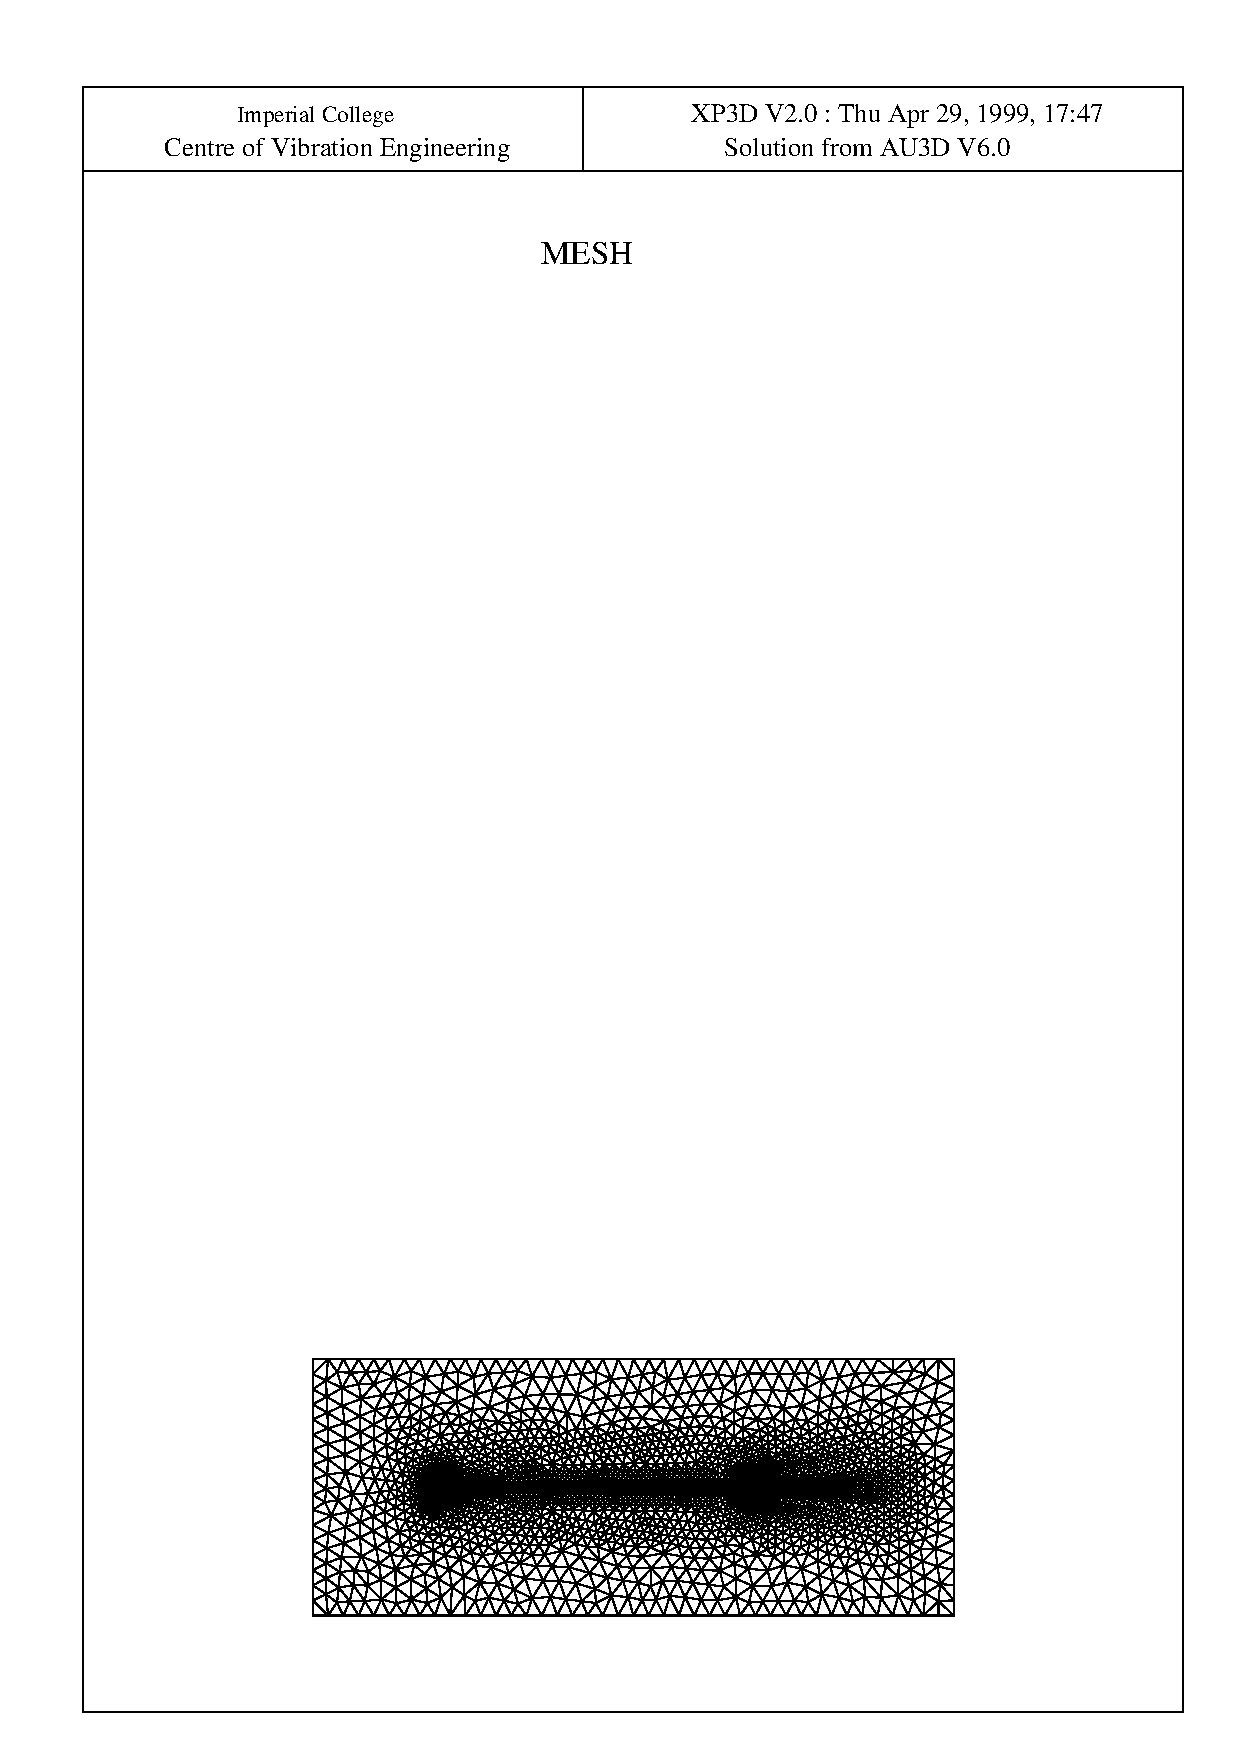
\includegraphics[width=80mm,clip=t]{CHAP_LINEAR/FIGURE/flat_laminar_mesh1.pdf}
       \hspace{0mm}} &
    \subfigure[trailing edge]
      {\hspace{0mm}
        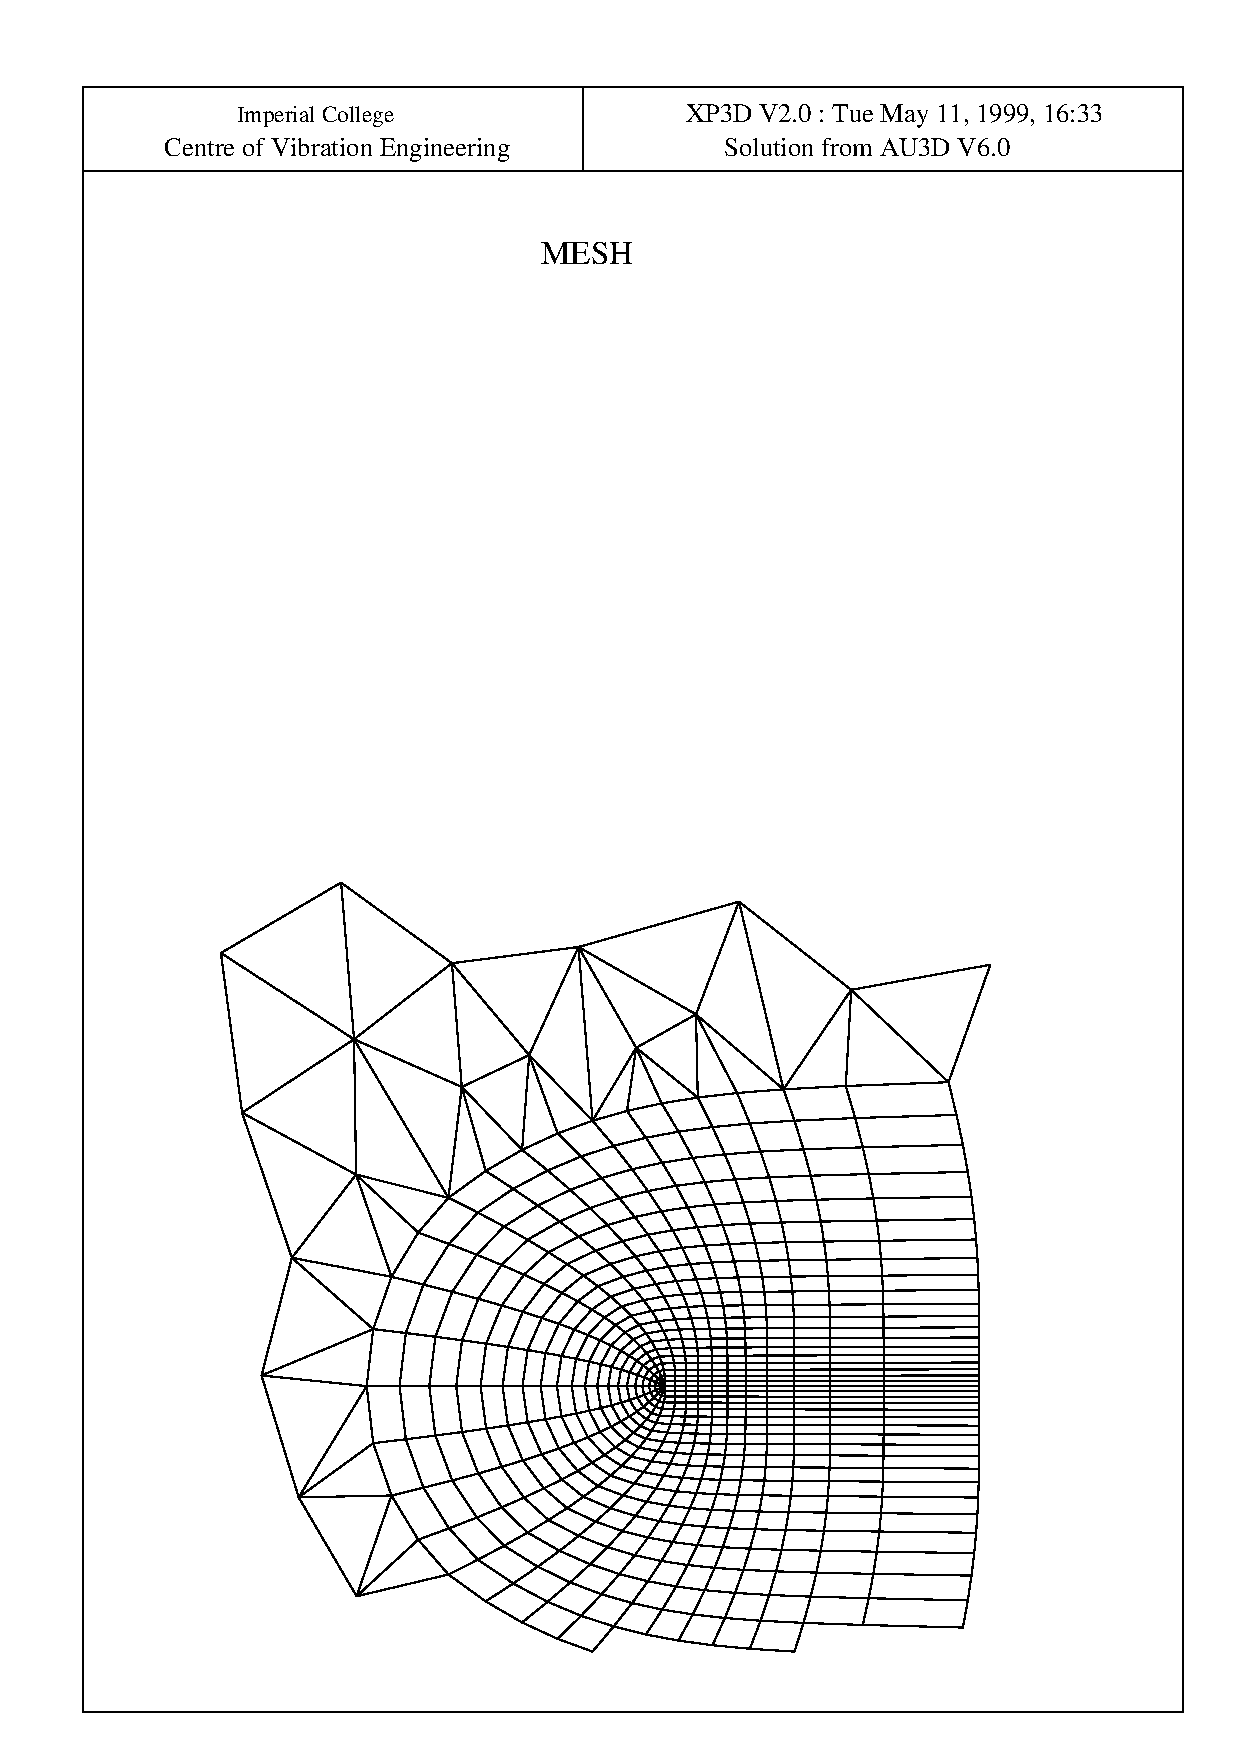
\includegraphics[width=40mm,clip=t]{CHAP_LINEAR/FIGURE/flat_laminar_mesh2.pdf}}
   \end{tabular}
 \end{center}
 \vspace{-7mm}
 \caption{Computational domain for laminar flow over a flat plate cascade}
 \label{flat_laminar_linear_mesh.fig}
\end{figure}
%
 This test case studies an unsteady laminar
 boundary layer with fluctuations in external velocity.
 The computational mesh is shown in Fig. \ref{flat_laminar_linear_mesh.fig}.
 The boundary layer region is discretised using 15 layers of quadrilateral elements,
 while the rest of the domain consists of triangles.
 The pitch to chord ratio of this cascade is unity so that the flow is
 as close as possible to that over an isolated flat plate.
 The steady-state flow  over an unstaggered flat plate cascade was obtained for
 a Mach number of 0.2.  The freestream Reynolds number is 60,000. Such a case is
 well within the incompressible flow regime, thus enabling  a meaningful comparison
 with the Blasius solution.  Indeed, the computed steady-state  velocity profile and
 the skin friction coefficient are found to be in very good agreement with the
 incompressible laminar boundary layer theory of  Blasius (Fig. \ref{flat_laminar_steady.fig}).
 Once the steady-state flow has been validated, the next stage is to study a
 velocity perturbation of the form:

%
\beq
  u = \varepsilon u\sm{\infty} e\se{-i\omega t}
\eeq
%
 where $u\sm{\infty}$ is the freestream velocity and $\varepsilon$ a small value ($\ll 1$).
 The disturbance is along the plate, in the freestream direction, denoted by co-ordinate $x$.
 Lighthill's \citeyear{Lighthill:1} theory provides two asymptotic values for
 the unsteady skin friction coefficient, one for very small and the other for very
 large reduced frequency values. Fig. \ref{flat_laminar_linear_sol.fig}a
 shows the wall shear stress amplitude variation with reduced frequency $\omega x/u\sm{\infty}$
 while Fig. \ref{flat_laminar_linear_sol.fig}b shows the computed phase angle
 between shear stress and external velocity. As expected, the computed results
 become asymptotic for the limiting cases of very small and very large reduced
 frequency. Similar comparisons between numerical results and Lighthill's theory
 are also reported by Cebeci \citeyear{Cebeci:1}.
%
%
%
\begin{figure}
  \begin{center}
  \begin{tabular}{c}
    \subfigure[Velocity profile]
       {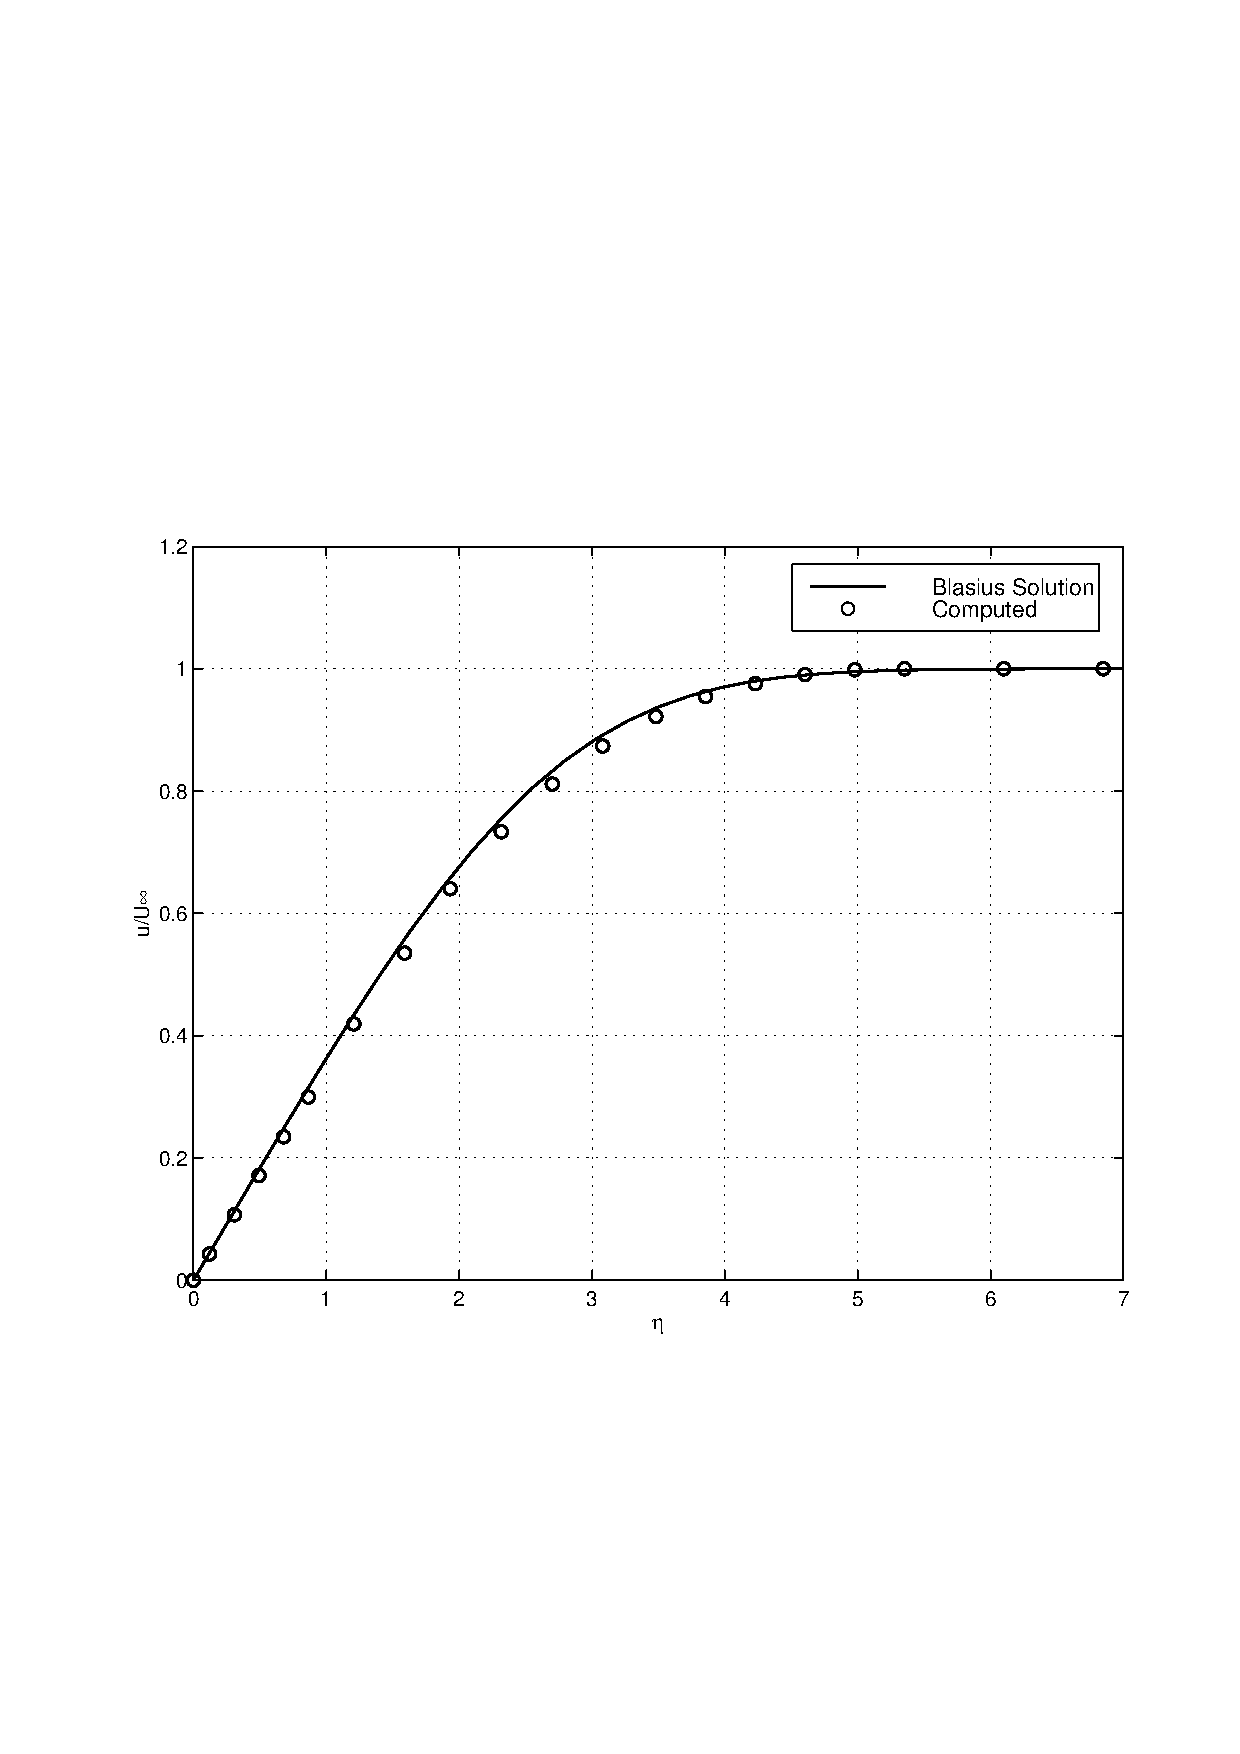
\includegraphics[width=110mm,clip=t]{CHAP_LINEAR/FIGURE/flat_laminar_vel.pdf}
       \hspace{0mm}} \\
    \subfigure[Skin friction coefficient]
      {\hspace{0mm}
        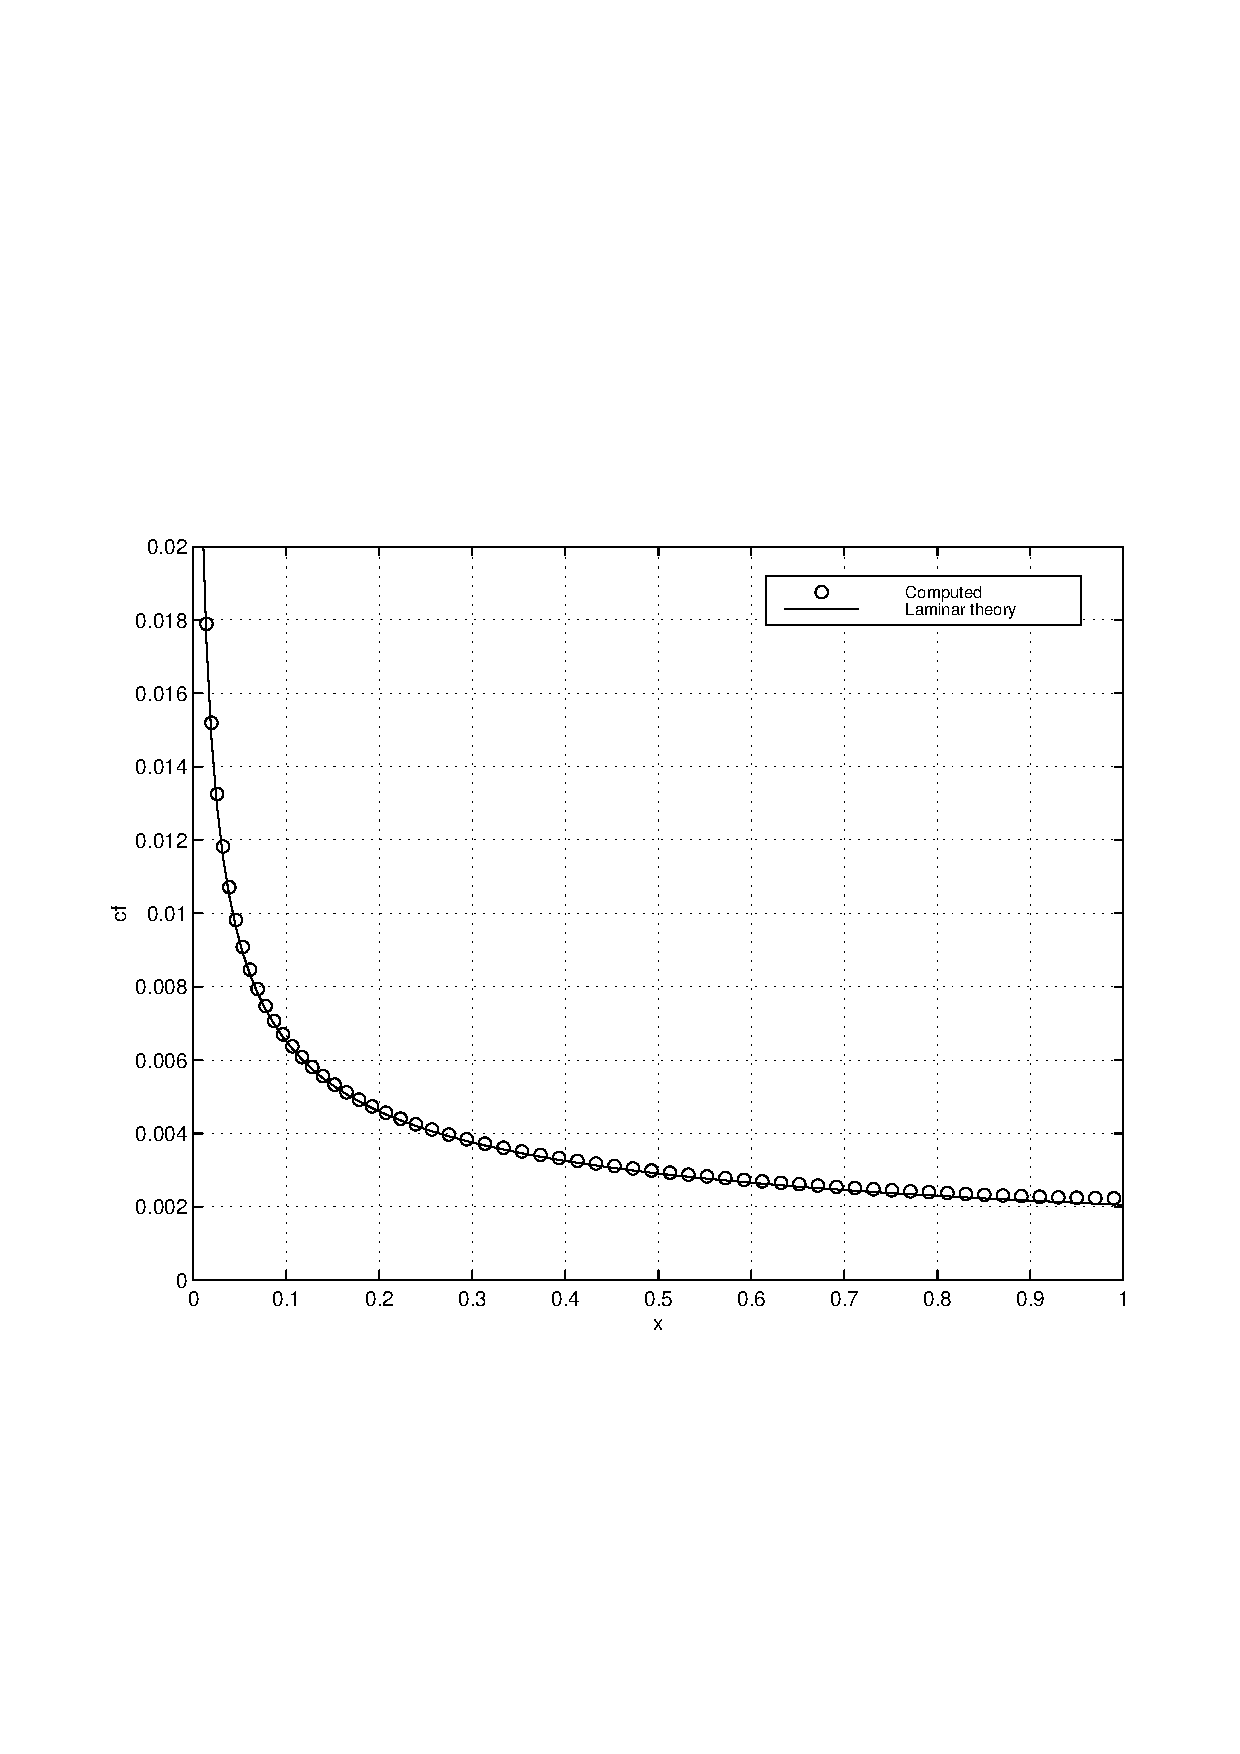
\includegraphics[width=110mm,clip=t]{CHAP_LINEAR/FIGURE/flat_laminar_cff.pdf}}
   \end{tabular}
 \end{center}
 \vspace{-7mm}
 \caption{Steady laminar flow over a cascade of flat plates}
 \label{flat_laminar_steady.fig}
\end{figure}
%
\begin{figure}
  \begin{center}
   \begin{tabular}{c}
    \subfigure[Amplitude]
       {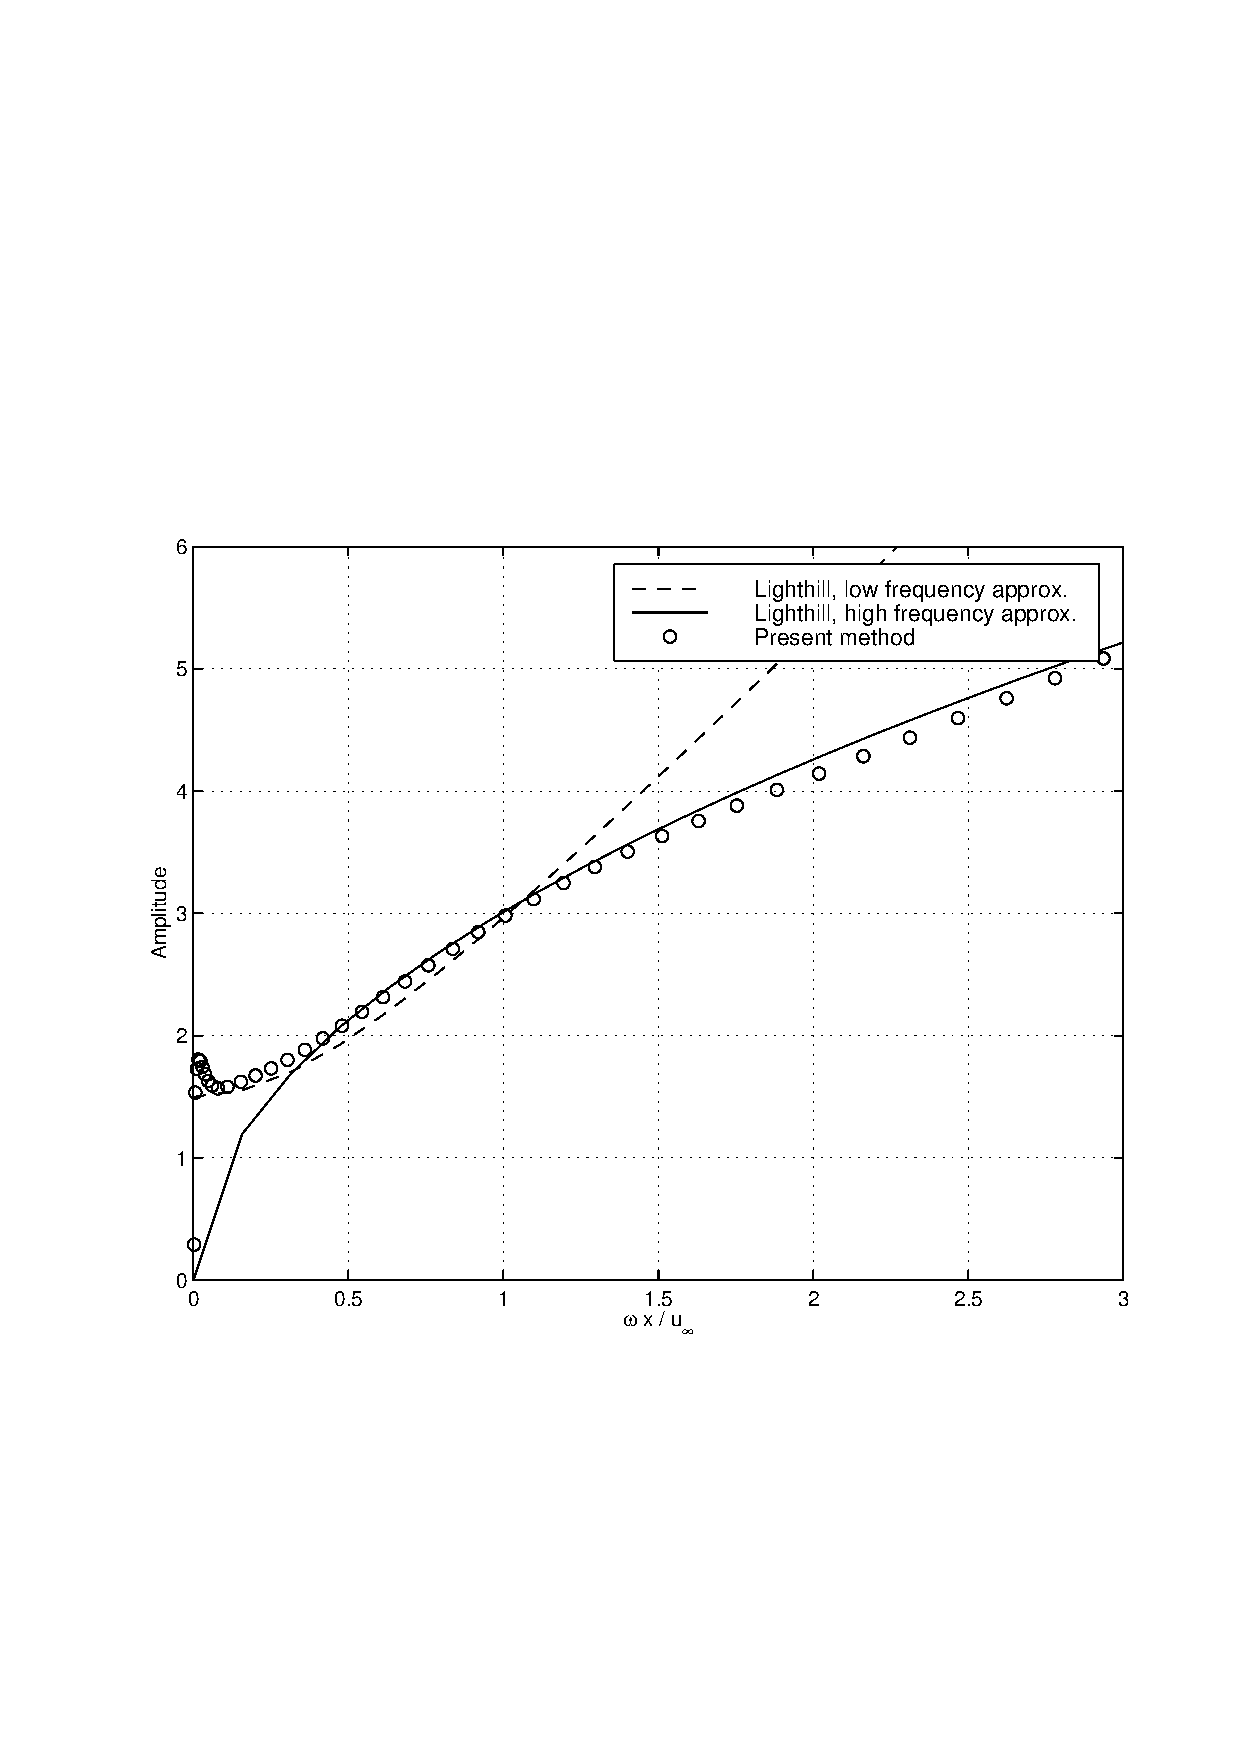
\includegraphics[width=110mm,clip=t]{CHAP_LINEAR/FIGURE/flat_laminar_ampli.pdf}
       \hspace{0mm}} \\
    \subfigure[Phase angle with respect to external velocity fluctuation]
      {\hspace{0mm}
        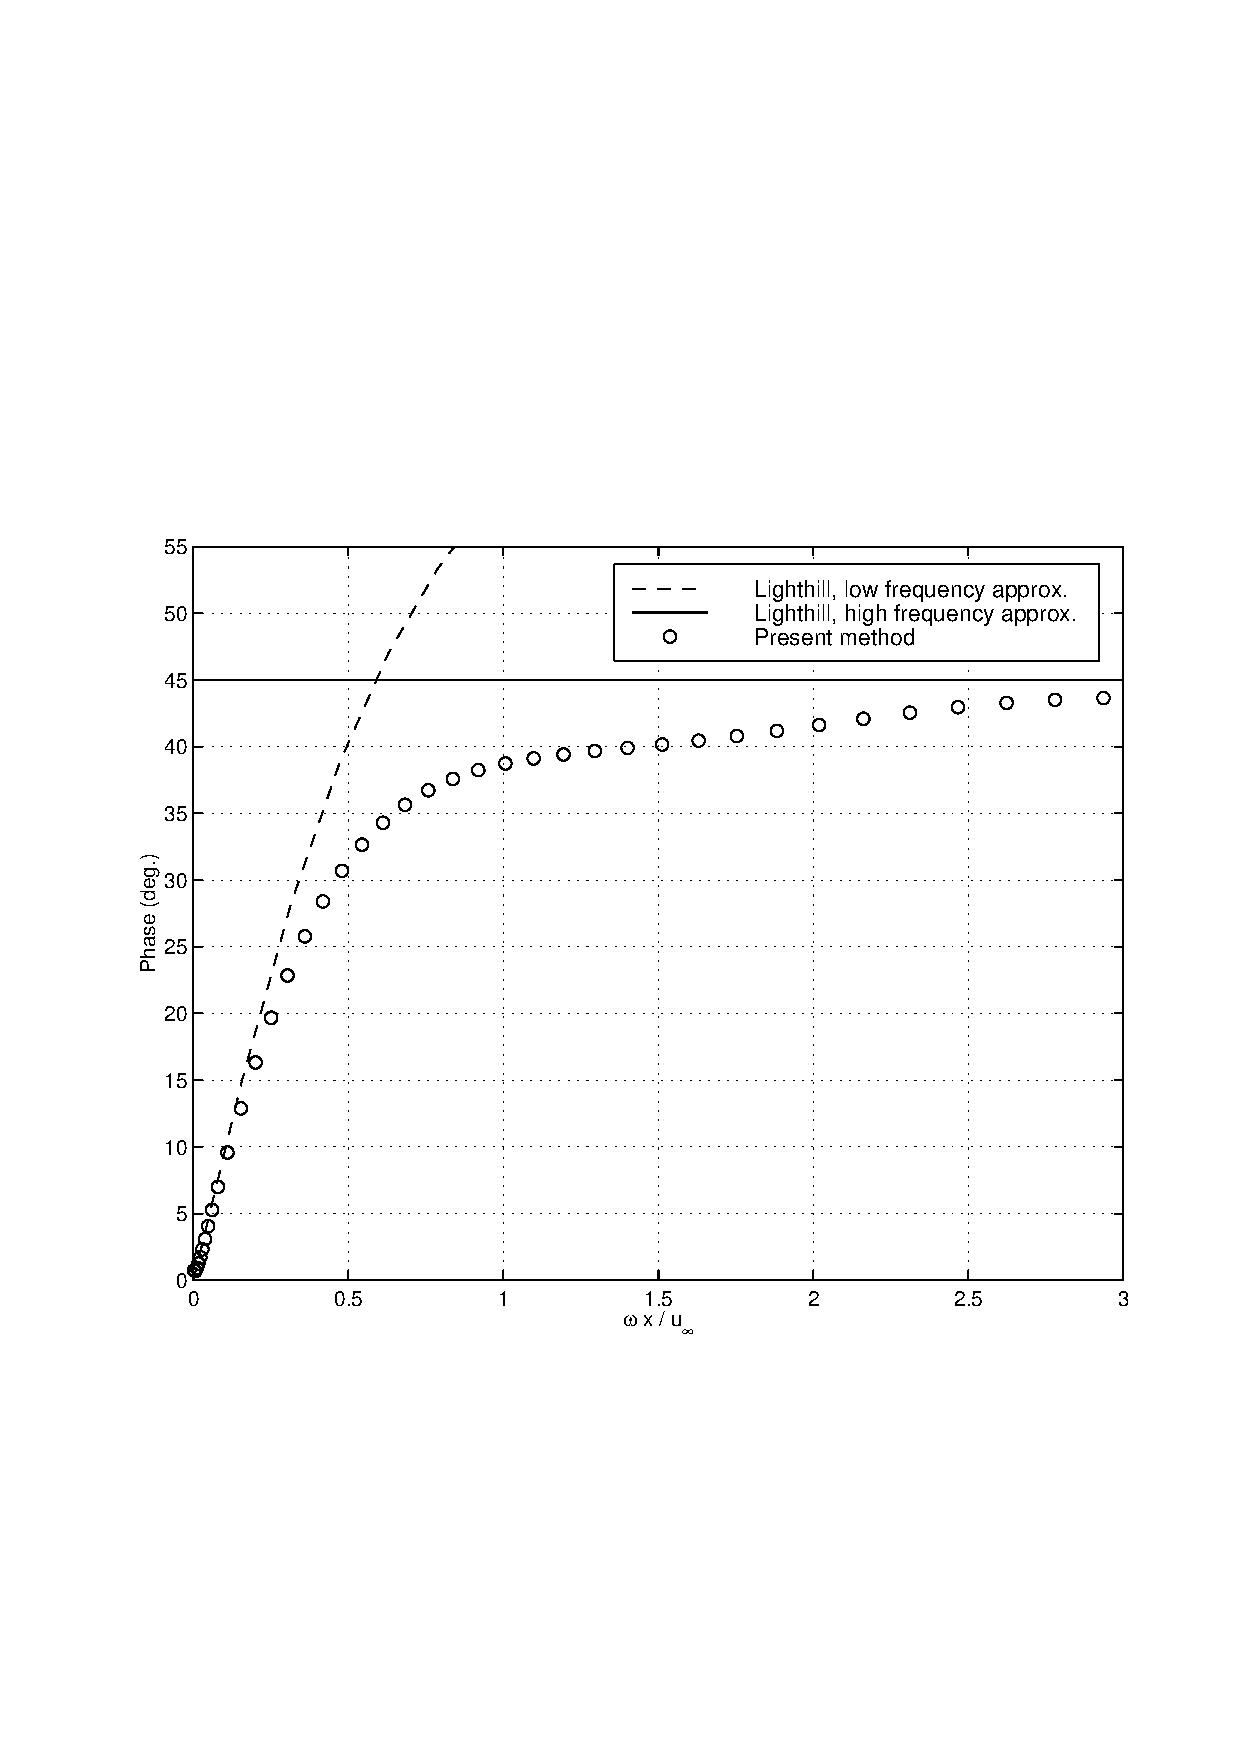
\includegraphics[width=110mm,clip=t]{CHAP_LINEAR/FIGURE/flat_laminar_phase.pdf}}
   \end{tabular}
 \end{center}
 \vspace{-7mm}
 \caption{Unsteady wall shear stresses for an oscillating laminar boundary layer}
 \label{flat_laminar_linear_sol.fig}
\end{figure}
%
